\section{Evaluation}

\subsection{Experimental Setup}

\textbf{Implementation of algorithms.}
The algorithms were implemented in C++ code.
It is built on top of \texttt{einsum\_ir} for the algorithm and uses \texttt{torch} for the test setups.
The contractions are hard-coded in the current implementation.

\textbf{Platform.}
The algorithms were tested on a server with an Nvidia Grace CPU Superchip in the Uni Jena and on an AWS g8c.metal-48xl Graviton instance.
All programs were compiled and executed with \texttt{g++} and \texttt{MPICH}.

\textbf{Measurements.}
All measurements show the average result of 10 contractions for each size.
I used Python Matplotlib\cite{matplotlib} to visualize the results.


\subsection{Distributed einsum\_ir Performance}

\begin{figure}[ht]
  \centering{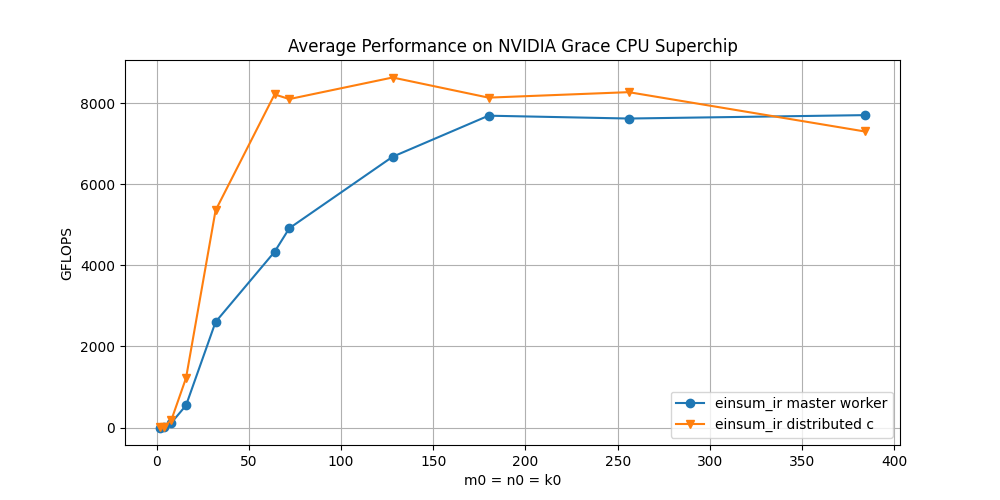
\includegraphics[width=1\textwidth]{gflops_grace_master_worker.png}
  }
  \caption{
    Performance of \texttt{einsum\_ir} distributed c algorithm and the master worker algorithm on a dual socket NVIDIA Grace CPU Superchip.
    The contraction is $c_0m_0k_0k_1m_1, c_0n_0k_0n_0n_1 \rightarrow c_0m_0n_0n_1m_1$ with $|c_0|=2$, $|m_0|=|n_0|=|k_0|$ and $|m_1|=|n_1|=|k_1|=70$.
    Grace has 72 cores per NUMA domain.
    }
  \label{fig:master_worker_perf}
\end{figure}

First we compare the performance of the master-worker algorithm with the distributed c algorithm.
We evaluate these algorithms on the einsum expression $c_0m_0k_0k_1m_1, c_0n_0k_0n_0n_1 \rightarrow c_0m_0n_0n_1m_1$.
Figure \ref{fig:master_worker_perf} shows, that the distributed c algorithm performs significantly better than the master-worker algorithm especially for small tensors.
This is expected since the distributed c algorithm performs no communication and thus is not slowed down on small tensors by a low compute intensity which implies being memory bound.
Its advantages diminish the higher the compute intensity is, as seen from $|m_0|=|n_0|=|k_0|= 180$ and onwards.
At $|m_0|=|n_0|=|k_0|= 384$ the master-worker algorithm even performs better than the distributed c algorithm.
I could not test larger sizes as the messages got to big for MPI, which uses a 32-bit signed integer for the element count and due to time constraints I could not rewrite the methods to send multiple smaller messages instead.
The overall result still shows the greater potential in a distributed algorithm, as it can scale easier to more nodes and performs better on most sizes, at least those I could test.
It also places fewer restrictions on the contraction itself as the c dimensions do not have to be the outermost dimension of all tensors.


\begin{figure}[ht]
  \centering{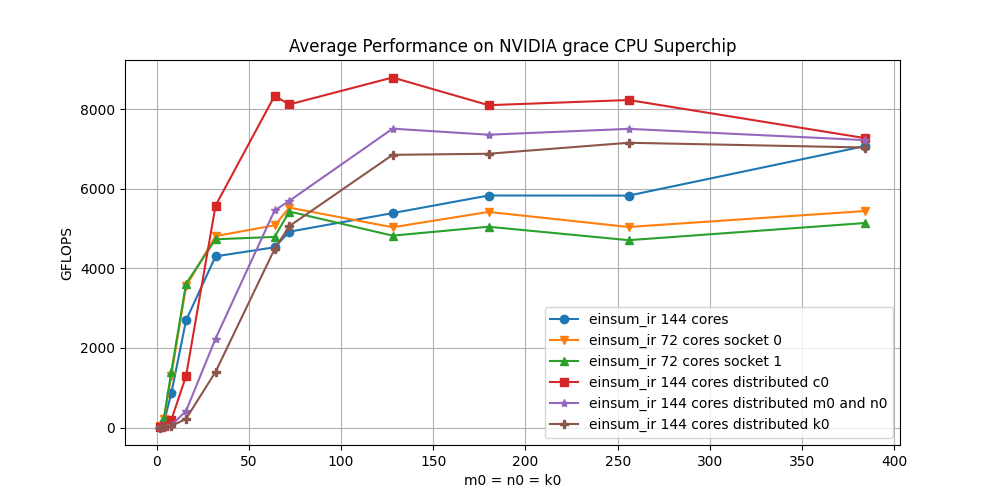
\includegraphics[width=1\textwidth]{gflops_grace.png}
  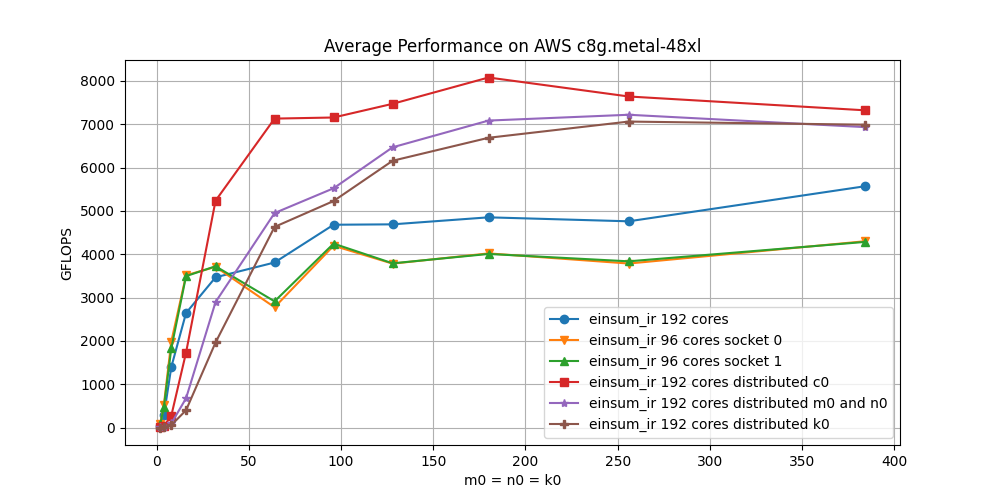
\includegraphics[width=1\textwidth]{gflops_g8c.png}
  }
  \caption{
    Performance of \texttt{einsum\_ir} on a dual socket NVIDIA Grace CPU Superchip and on a dual socket g8c.metal-48xl Graviton AWS instance.
    The contraction is $m_0c_0k_0k_1m_1, n_0c_0k_0n_0n_1 \rightarrow m_0n_0c_0n_1m_1$ with $|c_0|=2$, $|m_0|=|n_0|=|k_0|$ and $|m_1|=|n_1|=|k_1|=70\text{ on Grace and } 94\text{ on Graviton}$.
    Grace has 72 cores per NUMA domain; Graviton has 96.
    }
  \label{fig:einsum_ir_perf}
\end{figure}

Next we should compare the more general distributed algorithms against the base implementation.
For that we will look at the results in Figure \ref{fig:einsum_ir_perf}.
For tensors larger than $|m_0|=|n_0|=|k_0|=128$ we see significant performance improvements of the new distributed memory algorithms over the base shared memory implementation on both Grace and Graviton, except for $|m_0|=|n_0|=|k_0|=384$ on Grace where \texttt{einsum\_ir} matches the distributed performance.
We also note that for small tensors the distribution harms the performance, which suggests that small enough tensors should be locally contracted on only one process and then the results get distributed.
We also observe that in general the distributed c algorithm performs significantly better than both the distributed m and n and the distributed k algorithm, which are quite close in performance to each other with the distributed k one being a bit worse.
This is expected since the distributed c algorithm is the only one of the three algorithms to not have any communication happening and thus never having to run idle waiting for new data and no synchronization overheads.
The k algorithm is likely slightly slower than the m and n one, since it has double the amount of steps and with that also double the amount of synchronization happening.

Another thing we should specifically note on Grace is that the second socket performs about 5\% worse than first socket.
I am not sure why this is happening, but I should also note that in an earlier measurement all algorithms performed significantly worse on Grace.
The difference between those first measurements and the final ones were mainly length.
The first measurements comprised 100 runs for each contraction for all sizes $|m_0|=|n_0|=|k_0|=2,4,...,128$, which made the test runs significantly longer, taking multiple hours each.
One hypothesis for the worse performance would be bad cooling on specifically Grace's second socket.
The inclusion of the AWS Graviton instance should show that the algorithms perform well and that the bad initial performance on the Grace server was an outlier.


